\documentclass{beamer}
\input{themes/packages.tex}
\usetheme{apertus}

\title{\textbf{GSoC Phase I} : First Half \\ 
		\textbf{Project} : AXIOM Remote - Bootloader improvement and extension} 
\titlegraphic{
\includegraphics[width=10cm]{images/apertus_logo.png}}
\author{Priya Pandya}
\date

\begin{document}
{
    \setbeamertemplate{footline}{} 
    \frame{\titlepage}
}

\section*{Outline}

\begin{frame}{Outline}
    \tableofcontents
\end{frame}

\section{Phase I}

\begin{frame}[plain]
    \begin{beamercolorbox}[sep=8pt,center,shadow=true,rounded=true]{title}
        \usebeamerfont{title}\insertsectionhead\par
        \color{apertus_orange}\noindent\rule{10cm}{1pt}
        %\LARGE{\faFileTextO}
    \end{beamercolorbox}
\end{frame}

\subsection{Tasks}

\begin{frame}{Tasks}
	\begin{itemize}
		\item Task1: Flashing of firmware on PIC16s using PIC32
		\item Task2: PIC32 self-programming
	\end{itemize}
\end{frame}

\subsection{Task1}

\begin{frame}{Task1: Flashing of firmware on PIC16s using PIC32}
	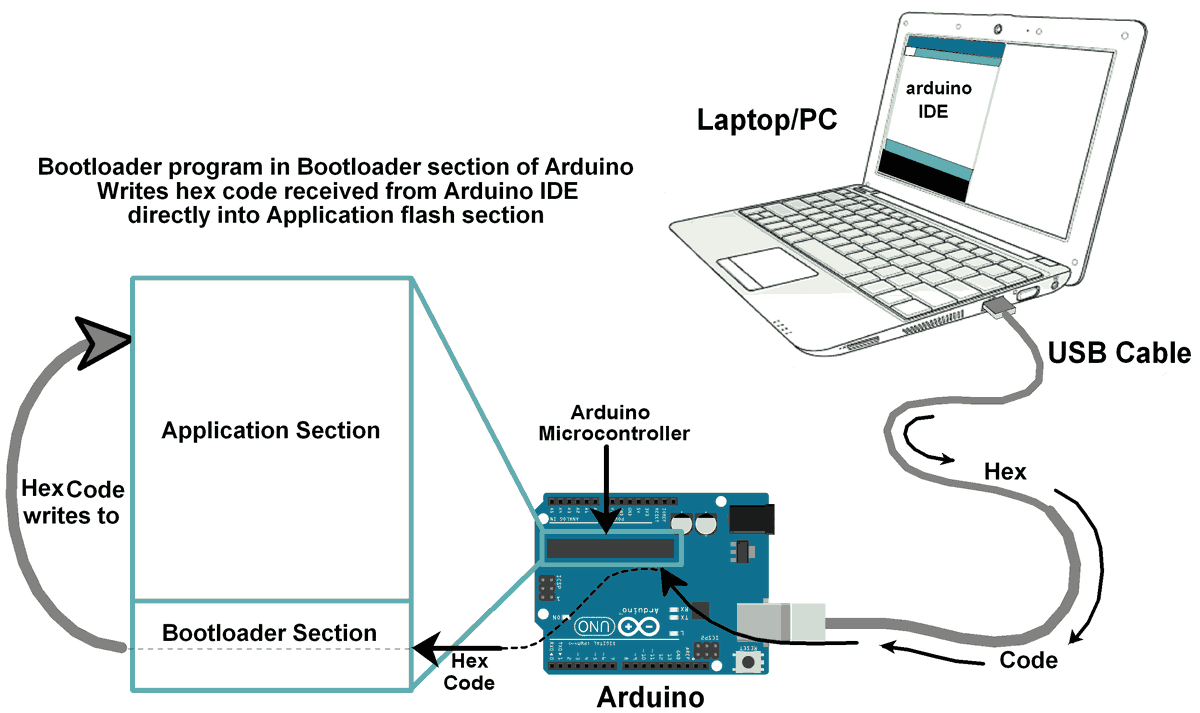
\includegraphics[width=8cm, center]{images/task1.png}
\end{frame}

\begin{frame}{Host PC}
	\begin{itemize}
		\item A python script will be used on the host PC (skeleton is ready)
		\item The features are:
			\begin{itemize}
				\item It uses pySerial module
				\item Command line arguments for operation, to select chip, to select UART port, to select HEX file
				\item It communicates with the Bootloader using \href{https://github.com/apertus-open-source-cinema/AXIOM-Remote/tree/dev/Firmware}{an ASCII based protocol}
			\end{itemize}
	\end{itemize}
\end{frame}

\begin{frame}{1 PICKit, 3 PICs? How?}
	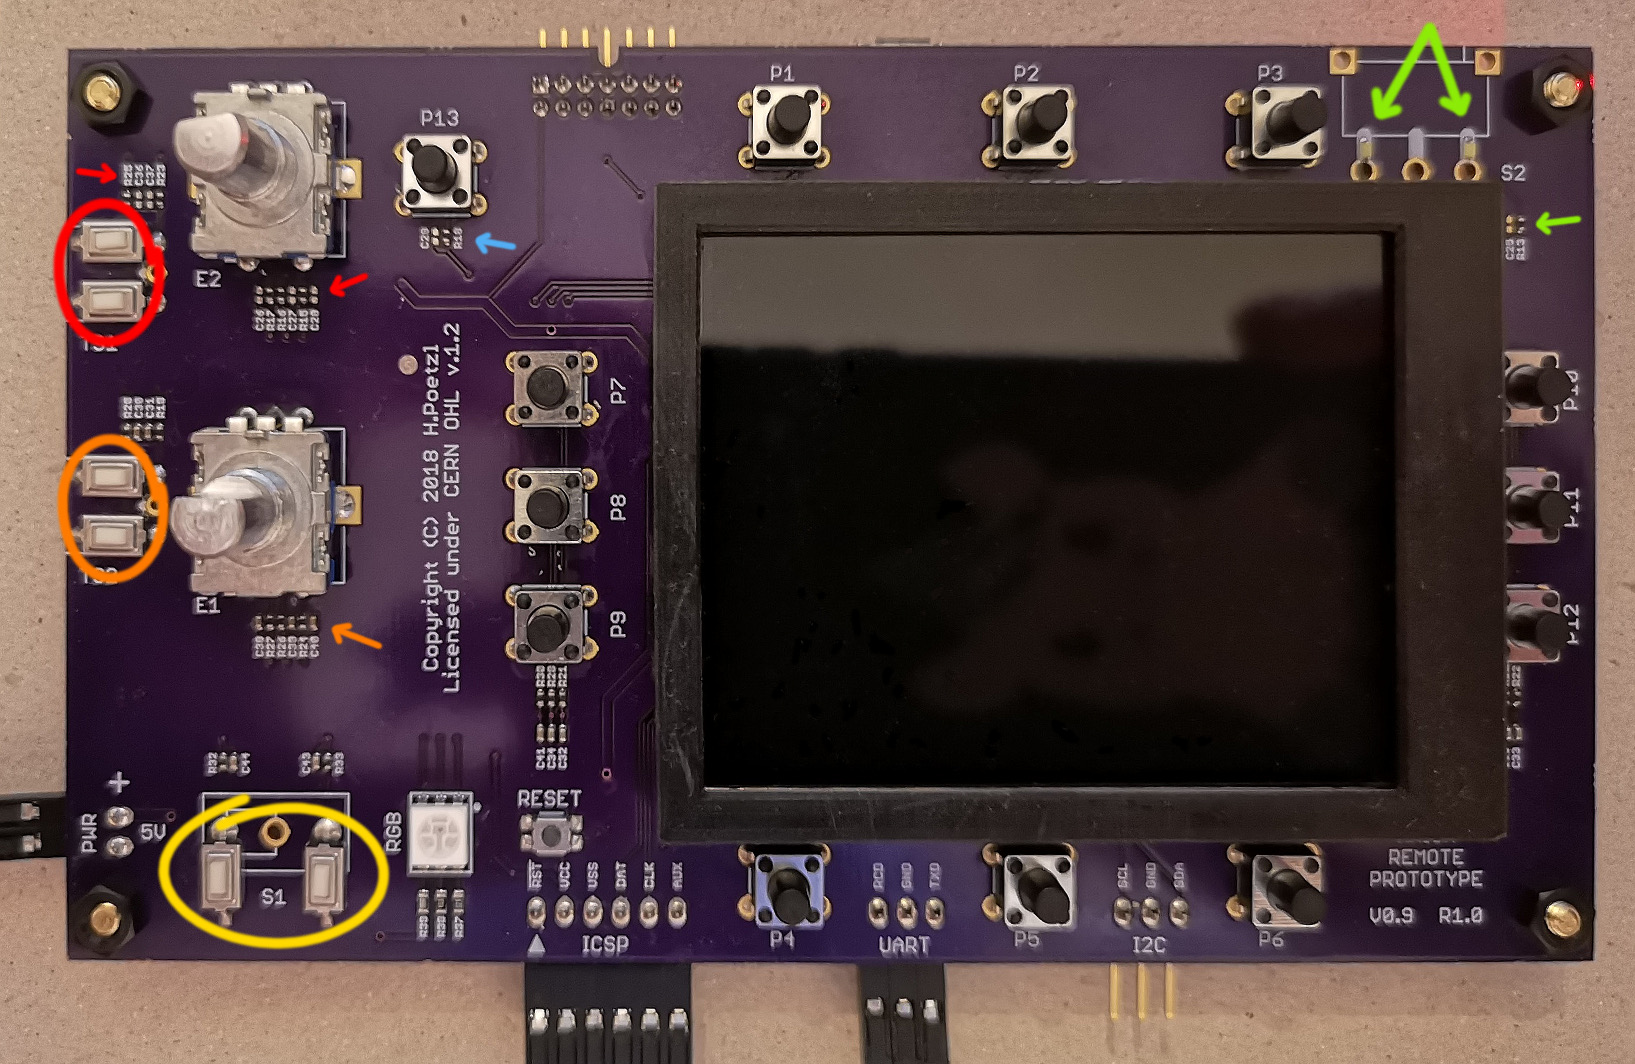
\includegraphics[width=6cm, left]{images/new_remote_prototype.jpg}

	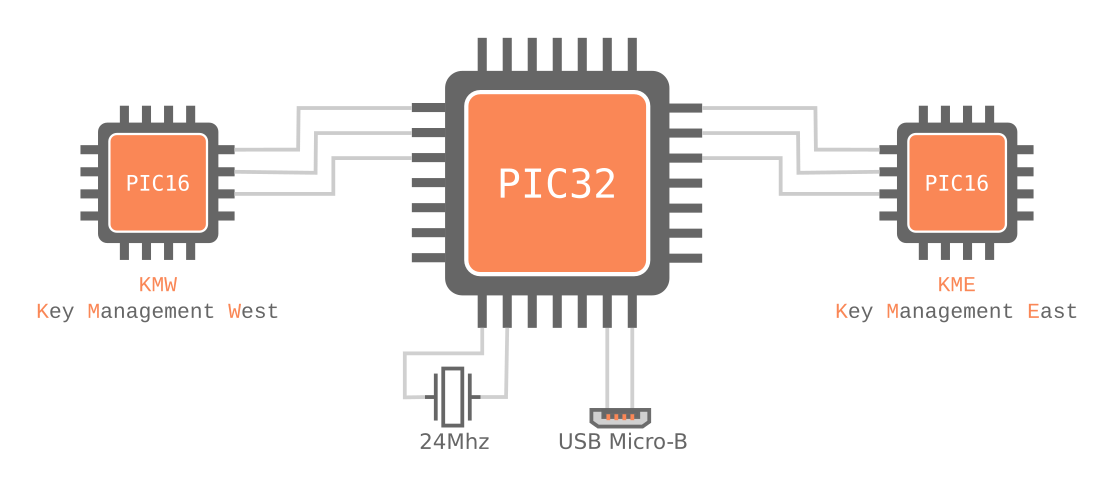
\includegraphics[width=6cm, right]{images/AXIOM_Remote_schematic.png}
\end{frame}

\begin{frame}{Solution : ICSProgrammer class}
	\begin{itemize}
		\item It replicates the functionality of a PICKit to communicate with the PIC16s (or KMs)
		\item It has all the ICSP commands defined there and simple read and write methods
	\end{itemize}
\end{frame}

\subsection{Task2}

\begin{frame}{Task2: PIC32 self-programming}
	\begin{itemize}
		\item To flash the firmware with UI in the PIC32
		\item Same python script and the protocol to communicate with the BL will be used
	\end{itemize}	
\end{frame}

\subsection{Plans for upcoming weeks}

\begin{frame}{Plans for upcoming weeks}
	\begin{itemize}
		\item This week:
			\begin{itemize}
				\item Create commands to read the data from Bootloader
			\end{itemize}
		\item If above successful then develop for write also
	\end{itemize}		
\end{frame}
\end{document}
